\documentclass[a4paper,11pt]{article}
%@@@@@@@@@@@@@@@@@@@@@@@@@@@@@@@@@@@@@@@@@@@@@@@@@@@@@@@@@@@
%@@@@@@@@@@@@@@@@      PACOTES BÁSICOS		     @@@@@@@@@@
%@@@@@@@@@@@@@@@@@@@@@@@@@@@@@@@@@@@@@@@@@@@@@@@@@@@@@@@@@@@

\usepackage[T1]{fontenc}
\usepackage[utf8]{inputenc}
\usepackage{lmodern} 
\usepackage[portuguese]{babel}
\usepackage{amsmath}
\usepackage{array}
\usepackage{graphicx}				%para imagens
\usepackage{epstopdf} 				%resolve problemas eps-pdf
\usepackage{pict2e}				%%writting to images
%@@@@@@@@@@@@@@@@@@@@@@@@@@@@@@@@@@@@@@@@@@@@@@@@@@@@@@@@@@@
%@@@@@@@@@@@@@@@@     PACOTES NÃO TAOBÁSICOS		 @@@@@@@@@@
%@@@@@@@@@@@@@@@@@@@@@@@@@@@@@@@@@@@@@@@@@@@@@@@@@@@@@@@@@@@
\usepackage{fancyhdr}				% para o cabeçalho bonito
\usepackage{caption}					%para legendas
\usepackage{subcaption}				% e sublegendas
\usepackage{placeins} 				%controlar o lugar dos floats
\pagestyle{fancy} 					% número de pag e cabeçalho
\usepackage{txfonts} 				%fontes bonitas? acho que para o título
\usepackage[usenames]{color} 		% algo com gunplot e eps
\usepackage{ifthen}
\usepackage{xparse}
\graphicspath{{./../images/}{./../data/}{./graph/}}	% procura imagens nessa pasta
\usepackage{float} %%para definir ambiente gráfico
\newfloat{Gráfico}{hbtp}{lop}[section]
%\usepackage{undertilde}	%%para notação de vetor do yuri
\usepackage[import]{xy} % para escrever em imagens
\xyoption{import}

\usepackage{listings}
\lstset{frame=single,}
%@@@@@@@@@@@@@@@@@@@@@@@@@@@@@@@@@@@@@@@@@@@@@@@@@@@@@@@@@@@
%@@@@@@@@@@@@@@@@      Cabeçalho de cada página      @@@@@@@
%@@@@@@@@@@@@@@@@@@@@@@@@@@@@@@@@@@@@@@@@@@@@@@@@@@@@@@@@@@@
\setlength{\headheight}{25pt}%compila sem erro
	\fancyhead{}
	\fancyfoot{}
	\fancyhead[R]{Sistemas de Medição}%direito superior
	\fancyhead[L]{
\includegraphics[height=0.25in]{./../images/logo_unb.pdf}}%esquerda superior
	\fancyfoot[C]{\thepage}%baixo centro
%E: Even page, O: Odd page, L: Left field, C: Center field, R: Right field, H: Header, F: Footer
% em documentos com dois lados use LO, RO. como esse documento não tem lados essa opção é inútil


%@@@@@@@@@@@@@@@@@@@@@@@@@@@@@@@@@@@@@@@@@@@@@@@@@@@@@@@@@@@
%@@@@@@@@@@@@@@@@      NOVOS COMANDOS		      @@@@@@@@@
%@@@@@@@@@@@@@@@@@@@@@@@@@@@@@@@@@@@@@@@@@@@@@@@@@@@@@@@@@@@
\newcommand\undermat[2]
	{
	  \makebox[0pt][l]
	  	{$\smash{\underbrace{\phantom{%
    \begin{matrix}#2\end{matrix}}}_{\text{$#1$}}}$
    		}#2
    	}
    	
\newcommand{\HRule}
	{
	\rule{\linewidth}{0.5mm}
	}
	
\newcommand{\EmptyPage}
	{
	\thispagestyle{empty}
	\mbox{ }
	\newpage	
	} 
	
\newcommand{\MakeMyTitlePage}[4]
%%Argumentos: 
%1º Nome da Matéria
%2º subtítulo ex: experimento IV
%3º título
%4º autores
% exemplo de autores:
%	\begin{center} \large
%		\begin{tabular}{llr} \
%		& & \\[0.05cm]		
%		Professora & Nadia Maria de Liz Koche & \\
%		
%		Alunos:& & \\
%		& Juarez A.S.F 					& 11/0032829\\
%		& Sérgio Fernandes da Silva Reis & 11/0140257\\
%		& Jedhai Pimentel				& 09/0007883\\	[0.05cm]	
%		\end{tabular}
%	\end{center}
{
\begin{titlepage}
\begin{center}

% Upper part of the page. The '~' is needed because \\
% only works if a paragraph has started.

\includegraphics[width=\textwidth]{./../images/logo_unb.pdf}~\\[1cm]

\Huge #1\\[0.5cm]

\huge #2

% Title
\HRule \\[0.4cm]
{ \huge \bfseries  #3}\\[0.4cm]

\HRule \\[0.5cm]

{\large \today}


\vfill %%o que vier depois vai ao fim da páginda


%Autor e Professor
\begin{center} \large
#4
\end{center}

\end{center}
\end{titlepage}

\EmptyPage
\tableofcontents
\newpage

}
	
%@@@@@@@@@@@@@@@@@@@@@@@@@@@@@@@@@@@@@@@@@@@@@@@@@@@@@@@@@@@
%@@@@@@@@@@@@@@@@      NOVOS AMBIENTES		      @@@@@@@@@
%@@@@@@@@@@@@@@@@@@@@@@@@@@@@@@@@@@@@@@@@@@@@@@@@@@@@@@@@@@@
\newcounter{graph-c}
\setcounter{graph-c}{0}


%\NewDocumentEnvironment{Graph}{m}
 % {%antes
  %\addtocounter{graph-c}{1}
  %\begin{figure}
  %}
 %{
 %depois
%	\end{figure} 
%	\caption*{Grafico \arabic{graph-c} - #1}
 %}

















%inclui todosos pacotes utilizados


\begin{document}

\begin{titlepage}
\begin{center}

% Upper part of the page. The '~' is needed because \\
% only works if a paragraph has started.

\includegraphics[width=\textwidth]{logo_unb.pdf}~\\[1cm]

\Huge Física Experimental 4\\[0.5cm]

\huge Experimento III

% Title
\HRule \\[0.4cm]
{ \huge \bfseries  Decaimento da Intensidade Luminosa e Coeficientes de Absorção e Reflexão}\\[0.4cm]

\HRule \\[0.5cm]

{\large \today}


\vfill %%o que vier depois vai ao fim da páginda


% Author and supervisor

	\begin{center} \large
		\begin{tabular}{llr} \
		& & \\[0.05cm]		
		Professora & Nadia Maria de Liz Koche & \\
		
		Alunos:& & \\
		& Juarez A.S.F 					& 11/0032829\\
		& Sérgio Fernandes da Silva Reis & 11/0140257\\
		& Jedhai Pimentel				& 09/0007883\\	[0.05cm]	
		\end{tabular}

	
	\end{center}


\end{center}
\end{titlepage}
\EmptyPage
\tableofcontents
\newpage

%@@@@@@@@@@@@@@@@@@@@@@@@@@@@@@@@@@@@@@@@@@@@@@@@@@@@@@@@@@@
%@@@@@@@@@@@@@@@@      OBJETIVOS      @@@@@@@@@@@@@@@@@@@@@@
%@@@@@@@@@@@@@@@@@@@@@@@@@@@@@@@@@@@@@@@@@@@@@@@@@@@@@@@@@@@
\section{Objetivos}
\paragraph{} Utilizar o interferômetro de Michelson para determinar o comprimento de onda de um laser e o índice de refração do ar à pressão de laboratório. 
%@@@@@@@@@@@@@@@@@@@@@@@@@@@@@@@@@@@@@@@@@@@@@@@@@@@@@@@@@@@
%@@@@@@@@@@@@@@@        MATERIAIS         @@@@@@@@@@@@@@@@@@
%@@@@@@@@@@@@@@@@@@@@@@@@@@@@@@@@@@@@@@@@@@@@@@@@@@@@@@@@@@@
\section{Materiais}
\paragraph{} O experimento faz uso de:
\begin{itemize}
	\item[•]Interferômetro de Michelson
	\item[•]Laser de He-Ne
	\item[•]Célula de pressão de 10mm
	\item[•]Bomba de vácuo manual
	\item[•]Lente com distância focal de 20 mm
	\item[•]Tela
\end{itemize} 

%@@@@@@@@@@@@@@@@@@@@@@@@@@@@@@@@@@@@@@@@@@@@@@@@@@@@@@@@@@@
%@@@@@@@@@@@@@@        INTRODUCAO       @@@@@@@@@@@@@@@@@@@@
%@@@@@@@@@@@@@@@@@@@@@@@@@@@@@@@@@@@@@@@@@@@@@@@@@@@@@@@@@@@
\newpage
\section{Introdução}
\paragraph{}Interferência é um fenômeno físico que ocorre quando duas ondas se superpõe. A onda resultante é a soma vetorial ponto a ponto das amplitudes das duas ondas iniciais. Se a onde 1 pode ser representada por $\psi_1(\utilde{x}, t)$ e 2 por $\psi_2(\utilde{x}, t)$ então a onda resultante é simplesmente $\psi_t = \psi_1(\utilde{x}, t) + \psi_2(\utilde{x}, t)$. Podem aqui ocorrer duas situações: a amplitude de $\psi_t$ é maior ou menor que a amplitude das duas ondas iniciais individualmente. No primeiro caso a interferência é dita construtiva, no segundo, destrutiva. A figura \ref{fig:intro-01} ilustra esse dois tipos de interferência. Esse fenômeno é portanto característico de ondas e sua ocorrência com feixes de luz indica a natureza ondulatória desta. 

\paragraph{}O objetivo do interferômetro é dividir um feixe coerente \footnote{todas as suas frentes de onda estão em fase} em dois, criar uma diferença de fase entre os dois e reuni-los novamente em um tela de captura. A diferença de fase entre os dois feixes pode ser feita basicamente de duas formas. Primeiramente pode-se alterar o caminho ótico percorrido pela luz, isso é feito alterando-se a distância percorrida. Além disso, assim como em uma corda de extremidade fixa, uma reflexão gerada quando a luz passe de um meio com menor índice de refração para um com maior causa uma inversão de fase. Para o estudo da interferência é vantajoso estudar a diferença de fase pelo número de comprimentos de onda percorridos. Dessa forma, o número de comprimentos de onda percorridos em um caminho homogêneo de comprimento \textbf{D} que sofre \textbf{r} reflexões é:
\begin{equation}
	n_t = n_D + n_r = \frac{D}{\lambda} +  r\frac{\lambda}{2}
\end{equation}
\paragraph{} Considere o esquema na figura \ref{fig:intro-02}. O laser representa uma luz coerente. A superfície \textbf{O} é o divisor de feixe e consiste em uma superfície semi-espelhada que permite que parte do feixe passe por ela e parte seja refletida. Digamos que \textbf{O} esteja a 45º com a direção definida pelo laser incidente, nesse caso os feixes divididos são perpendiculares. O feixe 1 da figura se divide em 2 e 3. O feixe 2 é gerado por reflexão na interface ar-espelho e sofre inversão de fase, o feixe 3 é gerado por transmissão e não altera a fase. O feixe 2 ao incidir em $M_2$ tem sua fase novamente invertida e volta a configuração inicial. O feixe 3 ao refletir em $M_1$ tem sua fase invertida. Parte do feixe 2' é transmitida por \textbf{O} e o feixe 2'' possui fase 0. Parte de 3' é transmitida para o vidro e é refletida na interface vidro-ar ao tentar sair. Essa reflexão ocorre numa interface onde a luz tenta ir de um alto índice de refração(vidro) para um baixo índice de refração(ar) e aqui não ocorre mudança de fase. Por isso 3'' mantêm a mesma fase de 3' e chega com meio comprimento de onda de diferença em relação a 2''. Nessa análise consideramos apenas feixes responsáveis pelo padrão de interferência. A figura \ref{fig:intro-03} focaliza a reflexão que causa as diferenças de fase resultantes. 
\paragraph{} Note que consideramos apenas as mudanças de fase devido a reflexão, ou seja, sem que haja mudança de caminho a diferença de fase já é de $\frac{\lambda}{2}$ e temos interferência destrutiva!

\paragraph{}Vamos considerar agora as diferença de fase causada por diferenças de caminho, para isso deixemos \textbf{M1} fixo e movamos \textbf{M2}. Veja que se \textbf{M2} se afasta em \textbf{d} o raio de luz terá sua trajetória adicionada em 2\textbf{d} uma vez que devem ser considerados os caminhos de ida e de volta. Sempre que a diferença de caminho total for de \textbf{$\lambda$} voltaremos a situação do destrutividade gerada pelas reflexões. Caímos então em interferência destrutiva caso:
\begin{equation}
	\triangle d = N \frac{\lambda}{2}
	\label{form-proced1}
\end{equation}


\paragraph{}Contando-se a variação nas franjas de interferência podemos usar essa equação para obter com muita precisão o comprimento de onda de uma onda estudo.

\paragraph{} Um outro modo de gerar diferença de fase entra os dois feixes é fazê-los percorrer mesmas distâncias porém em meios com índices de refração diferentes. Por exemplo podemos inserir no caminho de um feixe uma câmera de vácuo. Quando o ar for rarefeito teremos menos partículas por volume em média e o índice de refração deve ser mais baixo. Podemos estimar a variação de índice de refração do ar com a pressão pela forma linear:
\begin{equation}
	n(p) = n_{0} + \frac{\triangle n}{\triangle p}\cdot p
	\label{eq:n(p)}
\end{equation}

onde $n_0 \simeq 1$ é o índice de refração do ar quando a pressão é zero e $\frac{\triangle n}{\triangle p}$ é um coeficiente a ser determinado.

\paragraph{}Considere que na montagem do interferômetro tenhamos uma câmera de vácuo de comprimento \textbf{S} no percurso de apenas um dos feixes. A diferença de caminho ótico $\triangle x$ entre as duas ondas é causado exclusivamente pela diferença de índice de refração do ar dentro da câmera e do ar a pressão de laboratório.
\begin{equation}
	\begin{array}{lr}
		\triangle x = S(n(p + \triangle p) - n(p))  & \hspace{3 cm}(\div \triangle p) \\ \\
		\Rightarrow  \frac{\triangle x}{\triangle p} = \frac{S(n(p + \triangle p) - n(p))}{\triangle p}
	\end{array}
\end{equation}

\paragraph{} Quando sairmos de situação de interferência destrutiva para outra estamos andando $\lambda$. Quando andarmos \textbf{N} franjas teremos:
\begin{equation}
\frac{\triangle x}{\triangle p} = \frac{N \lambda}{\triangle p}
\label{eq:determinandocoeff}
\end{equation}


igualando as duas últimas igualdades e lembrando que o caminho \textbf{S} é multiplicado por dois pois a luz o transpassa 2 vezes obtemos:

\begin{equation}
 \frac{\triangle n}{\triangle p} = - \frac{N}{\triangle p} \cdot \frac{\lambda}{2S}
 \label{eq:achando-coeff}
\end{equation}

Essa equação nos da o coeficiente que precisávamos na fórmula \ref{eq:n(p)}. Pode-se então usar a fórmula \ref{eq:n(p)} para determinar o índice de refração do ar a pressão ambiente.

\FloatBarrier
\begin{figure}[H]
	\hspace{-1 cm}
	\begin{subfigure}[!htp]{0.4\textwidth}
		% GNUPLOT: LaTeX picture with Postscript
\begingroup
  \makeatletter
  \providecommand\color[2][]{%
    \GenericError{(gnuplot) \space\space\space\@spaces}{%
      Package color not loaded in conjunction with
      terminal option `colourtext'%
    }{See the gnuplot documentation for explanation.%
    }{Either use 'blacktext' in gnuplot or load the package
      color.sty in LaTeX.}%
    \renewcommand\color[2][]{}%
  }%
  \providecommand\includegraphics[2][]{%
    \GenericError{(gnuplot) \space\space\space\@spaces}{%
      Package graphicx or graphics not loaded%
    }{See the gnuplot documentation for explanation.%
    }{The gnuplot epslatex terminal needs graphicx.sty or graphics.sty.}%
    \renewcommand\includegraphics[2][]{}%
  }%
  \providecommand\rotatebox[2]{#2}%
  \@ifundefined{ifGPcolor}{%
    \newif\ifGPcolor
    \GPcolorfalse
  }{}%
  \@ifundefined{ifGPblacktext}{%
    \newif\ifGPblacktext
    \GPblacktexttrue
  }{}%
  % define a \g@addto@macro without @ in the name:
  \let\gplgaddtomacro\g@addto@macro
  % define empty templates for all commands taking text:
  \gdef\gplbacktext{}%
  \gdef\gplfronttext{}%
  \makeatother
  \ifGPblacktext
    % no textcolor at all
    \def\colorrgb#1{}%
    \def\colorgray#1{}%
  \else
    % gray or color?
    \ifGPcolor
      \def\colorrgb#1{\color[rgb]{#1}}%
      \def\colorgray#1{\color[gray]{#1}}%
      \expandafter\def\csname LTw\endcsname{\color{white}}%
      \expandafter\def\csname LTb\endcsname{\color{black}}%
      \expandafter\def\csname LTa\endcsname{\color{black}}%
      \expandafter\def\csname LT0\endcsname{\color[rgb]{1,0,0}}%
      \expandafter\def\csname LT1\endcsname{\color[rgb]{0,1,0}}%
      \expandafter\def\csname LT2\endcsname{\color[rgb]{0,0,1}}%
      \expandafter\def\csname LT3\endcsname{\color[rgb]{1,0,1}}%
      \expandafter\def\csname LT4\endcsname{\color[rgb]{0,1,1}}%
      \expandafter\def\csname LT5\endcsname{\color[rgb]{1,1,0}}%
      \expandafter\def\csname LT6\endcsname{\color[rgb]{0,0,0}}%
      \expandafter\def\csname LT7\endcsname{\color[rgb]{1,0.3,0}}%
      \expandafter\def\csname LT8\endcsname{\color[rgb]{0.5,0.5,0.5}}%
    \else
      % gray
      \def\colorrgb#1{\color{black}}%
      \def\colorgray#1{\color[gray]{#1}}%
      \expandafter\def\csname LTw\endcsname{\color{white}}%
      \expandafter\def\csname LTb\endcsname{\color{black}}%
      \expandafter\def\csname LTa\endcsname{\color{black}}%
      \expandafter\def\csname LT0\endcsname{\color{black}}%
      \expandafter\def\csname LT1\endcsname{\color{black}}%
      \expandafter\def\csname LT2\endcsname{\color{black}}%
      \expandafter\def\csname LT3\endcsname{\color{black}}%
      \expandafter\def\csname LT4\endcsname{\color{black}}%
      \expandafter\def\csname LT5\endcsname{\color{black}}%
      \expandafter\def\csname LT6\endcsname{\color{black}}%
      \expandafter\def\csname LT7\endcsname{\color{black}}%
      \expandafter\def\csname LT8\endcsname{\color{black}}%
    \fi
  \fi
  \setlength{\unitlength}{0.0500bp}%
  \begin{picture}(4534.00,3400.00)%
    \gplgaddtomacro\gplbacktext{%
      \csname LTb\endcsname%
      \put(946,815){\makebox(0,0)[r]{\strut{}-1}}%
      \put(946,1367){\makebox(0,0)[r]{\strut{}-0.5}}%
      \put(946,1920){\makebox(0,0)[r]{\strut{} 0}}%
      \put(946,2472){\makebox(0,0)[r]{\strut{} 0.5}}%
      \put(946,3025){\makebox(0,0)[r]{\strut{} 1}}%
      \put(1078,484){\makebox(0,0){\strut{} 0}}%
      \put(1588,484){\makebox(0,0){\strut{} 1}}%
      \put(2098,484){\makebox(0,0){\strut{} 2}}%
      \put(2608,484){\makebox(0,0){\strut{} 3}}%
      \put(3117,484){\makebox(0,0){\strut{} 4}}%
      \put(3627,484){\makebox(0,0){\strut{} 5}}%
      \put(4137,484){\makebox(0,0){\strut{} 6}}%
      \put(176,1919){\makebox(0,0){\strut{}$\psi(\utilde{x_0}, t)$}}%
      \put(2607,154){\makebox(0,0){\strut{}tempo}}%
    }%
    \gplgaddtomacro\gplfronttext{%
      \csname LTb\endcsname%
      \put(3150,2962){\makebox(0,0)[r]{\strut{}$\psi_1$}}%
      \csname LTb\endcsname%
      \put(3150,2742){\makebox(0,0)[r]{\strut{}$\psi_2$}}%
      \csname LTb\endcsname%
      \put(3150,2522){\makebox(0,0)[r]{\strut{}$\psi_t$}}%
    }%
    \gplbacktext
    \put(0,0){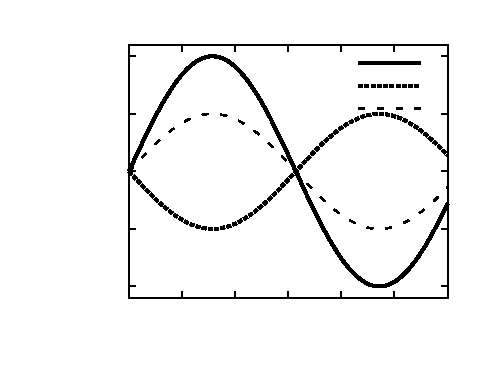
\includegraphics{intro-fig01}}%
    \gplfronttext
  \end{picture}%
\endgroup
	
		\caption{Interferência destrutiva}	
	\end{subfigure}	
		\hspace{3 cm}
	\begin{subfigure}[!htp]{0.5\textwidth}
		% GNUPLOT: LaTeX picture with Postscript
\begingroup
  \makeatletter
  \providecommand\color[2][]{%
    \GenericError{(gnuplot) \space\space\space\@spaces}{%
      Package color not loaded in conjunction with
      terminal option `colourtext'%
    }{See the gnuplot documentation for explanation.%
    }{Either use 'blacktext' in gnuplot or load the package
      color.sty in LaTeX.}%
    \renewcommand\color[2][]{}%
  }%
  \providecommand\includegraphics[2][]{%
    \GenericError{(gnuplot) \space\space\space\@spaces}{%
      Package graphicx or graphics not loaded%
    }{See the gnuplot documentation for explanation.%
    }{The gnuplot epslatex terminal needs graphicx.sty or graphics.sty.}%
    \renewcommand\includegraphics[2][]{}%
  }%
  \providecommand\rotatebox[2]{#2}%
  \@ifundefined{ifGPcolor}{%
    \newif\ifGPcolor
    \GPcolorfalse
  }{}%
  \@ifundefined{ifGPblacktext}{%
    \newif\ifGPblacktext
    \GPblacktexttrue
  }{}%
  % define a \g@addto@macro without @ in the name:
  \let\gplgaddtomacro\g@addto@macro
  % define empty templates for all commands taking text:
  \gdef\gplbacktext{}%
  \gdef\gplfronttext{}%
  \makeatother
  \ifGPblacktext
    % no textcolor at all
    \def\colorrgb#1{}%
    \def\colorgray#1{}%
  \else
    % gray or color?
    \ifGPcolor
      \def\colorrgb#1{\color[rgb]{#1}}%
      \def\colorgray#1{\color[gray]{#1}}%
      \expandafter\def\csname LTw\endcsname{\color{white}}%
      \expandafter\def\csname LTb\endcsname{\color{black}}%
      \expandafter\def\csname LTa\endcsname{\color{black}}%
      \expandafter\def\csname LT0\endcsname{\color[rgb]{1,0,0}}%
      \expandafter\def\csname LT1\endcsname{\color[rgb]{0,1,0}}%
      \expandafter\def\csname LT2\endcsname{\color[rgb]{0,0,1}}%
      \expandafter\def\csname LT3\endcsname{\color[rgb]{1,0,1}}%
      \expandafter\def\csname LT4\endcsname{\color[rgb]{0,1,1}}%
      \expandafter\def\csname LT5\endcsname{\color[rgb]{1,1,0}}%
      \expandafter\def\csname LT6\endcsname{\color[rgb]{0,0,0}}%
      \expandafter\def\csname LT7\endcsname{\color[rgb]{1,0.3,0}}%
      \expandafter\def\csname LT8\endcsname{\color[rgb]{0.5,0.5,0.5}}%
    \else
      % gray
      \def\colorrgb#1{\color{black}}%
      \def\colorgray#1{\color[gray]{#1}}%
      \expandafter\def\csname LTw\endcsname{\color{white}}%
      \expandafter\def\csname LTb\endcsname{\color{black}}%
      \expandafter\def\csname LTa\endcsname{\color{black}}%
      \expandafter\def\csname LT0\endcsname{\color{black}}%
      \expandafter\def\csname LT1\endcsname{\color{black}}%
      \expandafter\def\csname LT2\endcsname{\color{black}}%
      \expandafter\def\csname LT3\endcsname{\color{black}}%
      \expandafter\def\csname LT4\endcsname{\color{black}}%
      \expandafter\def\csname LT5\endcsname{\color{black}}%
      \expandafter\def\csname LT6\endcsname{\color{black}}%
      \expandafter\def\csname LT7\endcsname{\color{black}}%
      \expandafter\def\csname LT8\endcsname{\color{black}}%
    \fi
  \fi
  \setlength{\unitlength}{0.0500bp}%
  \begin{picture}(4534.00,3400.00)%
    \gplgaddtomacro\gplbacktext{%
      \csname LTb\endcsname%
      \put(946,815){\makebox(0,0)[r]{\strut{}-1}}%
      \put(946,1367){\makebox(0,0)[r]{\strut{}-0.5}}%
      \put(946,1920){\makebox(0,0)[r]{\strut{} 0}}%
      \put(946,2472){\makebox(0,0)[r]{\strut{} 0.5}}%
      \put(946,3025){\makebox(0,0)[r]{\strut{} 1}}%
      \put(1078,484){\makebox(0,0){\strut{} 0}}%
      \put(1588,484){\makebox(0,0){\strut{} 1}}%
      \put(2098,484){\makebox(0,0){\strut{} 2}}%
      \put(2608,484){\makebox(0,0){\strut{} 3}}%
      \put(3117,484){\makebox(0,0){\strut{} 4}}%
      \put(3627,484){\makebox(0,0){\strut{} 5}}%
      \put(4137,484){\makebox(0,0){\strut{} 6}}%
      \put(176,1919){\makebox(0,0){\strut{}$\psi(\utilde{x_0}, t)$}}%
      \put(2607,154){\makebox(0,0){\strut{}tempo}}%
    }%
    \gplgaddtomacro\gplfronttext{%
      \csname LTb\endcsname%
      \put(3150,2962){\makebox(0,0)[r]{\strut{}$\psi_1$}}%
      \csname LTb\endcsname%
      \put(3150,2742){\makebox(0,0)[r]{\strut{}$\psi_2$}}%
      \csname LTb\endcsname%
      \put(3150,2522){\makebox(0,0)[r]{\strut{}$\psi_t$}}%
    }%
    \gplbacktext
    \put(0,0){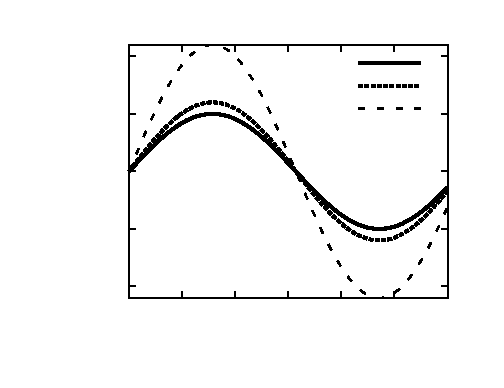
\includegraphics{intro-fig02}}%
    \gplfronttext
  \end{picture}%
\endgroup
	
		\caption{Interferência construtiva}
	\end{subfigure}	
	\caption{Diferentes formas de interferência}
	\label{fig:intro-01}
\end{figure} 
\begin{figure}[H]
	\hspace{-1 cm}
	\begin{subfigure}[!htp]{0.5\textwidth}
		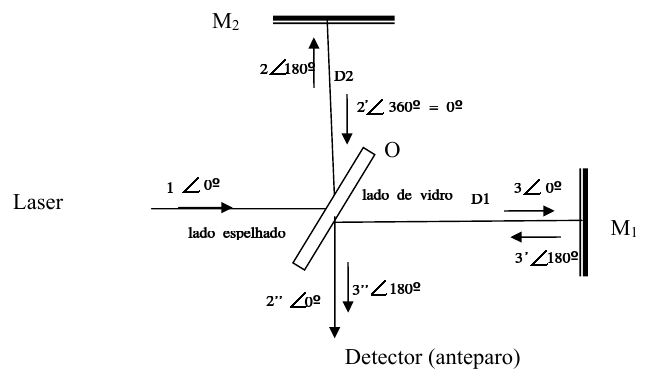
\includegraphics[scale=0.5]{./images/interferometro.png}
		\caption{Interferômetro de Michelson}
		\label{fig:intro-02}
	\end{subfigure}
	\hspace{2 cm}
	\begin{subfigure}[!htp]{0.5\textwidth}
		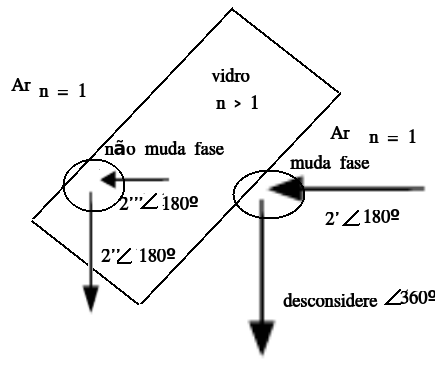
\includegraphics[scale=0.5]{./images/fig-intro03.png}
		\caption{Foco na interface de reflexão para o feixe 2}
		\label{fig:intro-03}
	\end{subfigure}
	\caption{Reflexões causam diferença de fase}
\end{figure}
\FloatBarrier

\newpage
%@@@@@@@@@@@@@@@@@@@@@@@@@@@@@@@@@@@@@@@@@@@@@@@@@@@@@@@@@@@
%@@@@@@@@@@@@       PROCEDIMENTOS        @@@@@@@@@@@@@@@@@@@
%@@@@@@@@@@@@@@@@@@@@@@@@@@@@@@@@@@@@@@@@@@@@@@@@@@@@@@@@@@@
\section{Procedimentos}
\paragraph{} Primeiramente ajusta-se o espelho divisor para que o feixe incidente o atinja em 45º.
Antes mesmo de colocar a lente ajusta-se os espelhos para que os dois pontos vermelhos causados pelas reflexões estejam
próximos. Colocamos a lente entre a fonte de laser e o espelho divisor e é feito um ajuste fino dos espelhos
procurando o formato de interferência na tela de captura. O ajuste deve ser feito ainda
de forma que a figura de interferência esteja no centro do \emph{spot} luminoso. Chamemos de espelho 1 aquele acoplado ao micrometro e 2 aquele de ajuste simples. A partir de agora o espelho 2 está fixo
e somente alteraremos o parafuso micrométrico do espelho 1. Ajusta-se o espelho 1 até que se obtenha uma figura de interferência
com centro escuro.  Nessa posição anota-se a medida do parafuso micrométrico, ela será considerada o zero das nossas medidas. 
Gira-se agora o parafuso sempre na mesma direção e a cada vinte aparições de centro escuro na figura de interferência anota-se
o valor medido no micrômetro. Deve-se ter em mente que a redução utilizada no sistema parafuso micrométrico é de 1:10, portanto
um incremente de 10 mm no parafuso corresponde um avança ou recuo de 1mm do espelho 1. Um gráfico d(N) vs N é feito. 

\paragraph{} Agora coloca-se a câmera de vácuo acoplada com bomba manual entre o espelho divisor e o espelho 2. Novamente o ajuste é feito de modo a 
visualizar a figura de interferência com centro escuro na tela. Reduz-se gradualmente a pressão na câmera e para cada novo centro escuro 
que obtermos anotamos o número de franjas observadas desde o início processo e a pressão manométrica. O processo é feito até que se atinja a menor 
pressão possível. As medidas são então refeitas para garantir confiabilidade dos dados. Entre uma medida e outra a câmera deve ser aberta e ventilada. Mede-se ainda a pressão atmosférica ambiente e o comprimento geométrico interno a câmera, se essa medida não for possível anota-se o valor
nominal do fabricante. A figura \ref{montagem} ilustra a montagem dos dois procedimentos.
\FloatBarrier
\begin{figure}[H]
	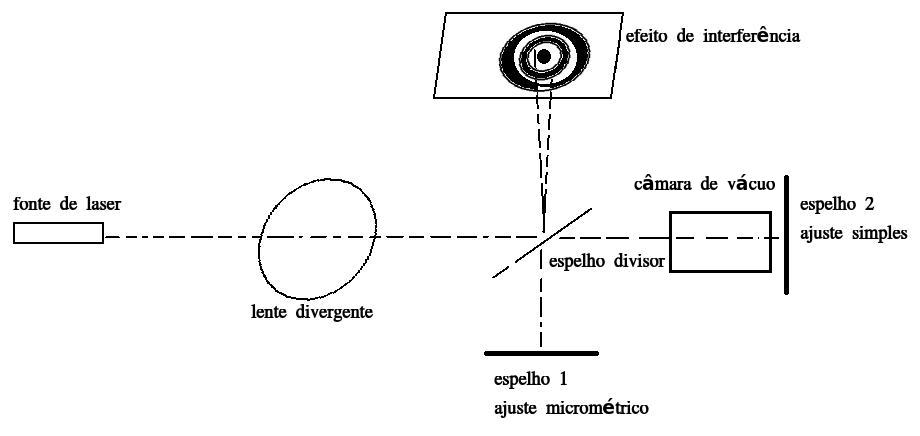
\includegraphics[scale=0.4]{./images/montagem.jpeg}
	\caption{Montagem do interferômetro}
	\label{montagem}
\end{figure}
\FloatBarrier
\newpage
%@@@@@@@@@@@@@@@@@@@@@@@@@@@@@@@@@@@@@@@@@@@@@@@@@@@@@@@@@@@
%@@@@@@@@@@@@@@@@@@@       DADOS      @@@@@@@@@@@@@@@@@@@@@@
%@@@@@@@@@@@@@@@@@@@@@@@@@@@@@@@@@@@@@@@@@@@@@@@@@@@@@@@@@@@

\section{Dados}

\paragraph{} Os dados do procedimento 1 são mostrados na tabela \ref{tab:proced1} e do 2º procedimento na tabela \ref{tab:proced2}
\FloatBarrier
\begin{table}[!htp]
	\centering
	\begin{tabular}{|l|l|}\hline
	n & d($\pm 0.00005$cm) \\ \hline
			 0 &  0.72800 \\ \hline 
		 20 &  0.73450 \\ \hline 
		 40 &  0.74100 \\ \hline 
		 60 &  0.74650 \\ \hline 
		 80 &  0.75300 \\ \hline 
		 100 &  0.75950 \\ \hline 
		 120 &  0.76600 \\ \hline 
		 140 &  0.77200 \\ \hline 
		 160 &  0.77850 \\ \hline 
		 180 &  0.78500 \\ \hline 
		 200 &  0.79050 \\ \hline 

	\end{tabular}
	\caption{Dados do procedimento 1}
	\label{tab:proced1}
\end{table}
\FloatBarrier
\FloatBarrier
\begin{table}[!htp]
\centering	
	\begin{tabular}{|l|l|l|}\hline
	n & $P_1 \pm 5mBar$ & $P_2 \pm 5mBar$ \\ \hline
			 1 &  -100 &  -120 \\ \hline 
		 2 &  -230 &  -240 \\ \hline 
		 3 &  -340 &  -370 \\ \hline 
		 4 &  -460 &  -480 \\ \hline 
		 5 &  -570 &  -600 \\ \hline 
		 6 &  -680 &  -720 \\ \hline 
		 7 &  -810 &  -840 \\ \hline 

	\end{tabular}
	\caption{Dados do procedimento 2}
	\label{tab:proced2}

\end{table}
\FloatBarrier
\paragraph{} A pressão atmosférica e o comprimento geométrico informado pelo fabricante da câmera de vácuo são:
\begin{equation}
\begin{array}{l}
	P_{\mbox{atm}} = 678.0 \mbox{mmHg} \pm 0.5\mbox{mm}\\
	S = 10 \mbox{mm}
\end{array}
\end{equation}
%@@@@@@@@@@@@@@@@@@@@@@@@@@@@@@@@@@@@@@@@@@@@@@@@@@@@@@@@@@@
%@@@@@@@@@@@@@@       Análise         @@@@@@@@@@@@@@@@@@@@@@
%@@@@@@@@@@@@@@@@@@@@@@@@@@@@@@@@@@@@@@@@@@@@@@@@@@@@@@@@@@@
\newpage
\section{Análise de Dados}
\paragraph{} Os dados da tabela \ref{tab:proced1} são plotados no gráfico \ref{graph-1}. A regressão da curva obtida é:

\begin{equation}
	\sin(\theta) = (0.0000011 \pm 0.0000001)\frac{1}{d}

\end{equation}

\paragraph{}Comparamos com a fórmula \ref{form-proced1} para obter o comprimento de onda da onda em estudo:
\begin{displaymath}
	\lambda = 2 * (0.000314 \pm 0.000001)mm  
\end{displaymath}

\begin{equation}
	\begin{tabular}{|c|}\hline
	$\lambda =  (628 \pm 2) nm$\\ \hline	
	\end{tabular}
\end{equation}



\paragraph{}A média dos dados do segundo procedimento é plotada no gráfico \ref{graph-2} e a regressão obtida é:

\begin{equation}
	N(p) = (0.031 \pm 0.028) + (-0.00847 \pm 0.00005) p

\end{equation}

O coeficiente angular dessa reta nos dá quanta franjas andamos por variação de pressão, portanto:
\begin{equation}
	\frac{\triangle N}{\triangle p} = - 0.00847 \pm 0.00005 \frac{1}{\mbox{mBar}}
\end{equation}

com esses dois dados temos:

\begin{displaymath}
	\frac{\triangle n }{\triangle p} = - \frac{\triangle N}{\triangle P} \cdot \frac{\lambda}{2S} = (0.00847 \pm 0.00005)\frac{1}{\mbox{mBar}} \cdot (628 \pm 2)\mbox{nm} \cdot \frac{1}{2 \cdot 10 \mbox{mm}}
\end{displaymath}

\begin{equation}
	\frac{\triangle n }{\triangle p} = (2.66 \pm  0.02)10^{-7} \frac{1}{\mbox{mBar}} 
	\label{coeff}
\end{equation}

\paragraph{}Onde a propagação do erro foi feito utilizando a fórmula:
\begin{displaymath}
	\triangle \left( \frac{\triangle n }{\triangle p} \right) = \frac{1}{2S} \cdot \left(\frac{\triangle N}{\triangle P} \triangle \lambda + \triangle \left(\frac{\triangle N}{\triangle P}\right) \lambda\right)
\end{displaymath}
A equação \ref{coeff} é justamente o coeficiente que precisávamos para usar a fórmula \ref{eq:n(p)}. Precisamos agora usar a pressão ambiente medida:
\begin{displaymath}
    P_{\mbox{amb}} = (670.0 \pm 0.5)\mbox{mmHg} = 890.4 \pm 0.7 \mbox{mbar}
\end{displaymath}
Onde o erro foi obtido por:
\begin{displaymath}
	\triangle P_{\mbox{mbar}} = \frac{1010\mbox{mbar}}{760 \mbox{mmHg}} \triangle P_{\mbox{mmHg}}
\end{displaymath}
\paragraph{}Obtemos finalmente o índice de refração do ar a pressão atmosférica ambiente:
\begin{displaymath}
    n_{\mbox{p$_{\mbox{amb}}$}} = n_0 + \frac{\triangle n}{\triangle p} \cdot p_{\mbox{amb}} = 1 + (2.66 \pm 0.02)10^{-7}\frac{1}{\mbox{mbar}} \cdot (890.4 \pm 0.7)\mbox{mbar}
\end{displaymath}

\begin{equation}
	\begin{tabular}{|c|}\hline
	$n_{\mbox{p amb}} = 1.000237 \pm 0.000002 $\\ \hline	
	\end{tabular}
\end{equation}

onde o erro foi calculado com a fórmula:
\begin{displaymath}
      \triangle n = p_{\mbox{amb}} \triangle \left( \frac{\triangle n}{\triangle p} \right) + \frac{\triangle n}{\triangle p} \triangle  \left( p_{\mbox{amb}} \right)
\end{displaymath}

\paragraph{}Para o comprimento de onda a razão erro-medida é de 3.2\% e para o índice de refração 0.0002\%.Nota-se que ambas as medidas obtidas, $\lambda$ e n, são muito precisas. Observando o caminho da propagação do erro vê-se que sua ordem se deve a grande precisão instrumental do parafuso micrométrico. Quanto a medida do $\lambda$, apesar de precisa, não se pode dizer que foi acurada, pois o valor nominal indicado pelo fabricante de 632 nm está fora da margem de erro. Alguns fatores podem ter contribuído para isso. Em primeiro lugar a contagem das franjas foi feita a olho nu e não se considerou um erro associado a essa medida. Além disso as medidas foram feitas uma única vez, não considerando portanto o erro aleatório. A repetição das medidas daria mais confiabilidade aos dados e mais um erro a ser considerado. Essas duas fontes de erro poderiam ser incluídas na propagação e poderiam resultar em uma margem de erro maior que englobasse o valor nominal.

\FloatBarrier
  

\begin{figure}

    \begin{subfigure}[!htp]{0.3\textwidth}
        % GNUPLOT: LaTeX picture with Postscript
\begingroup
  \makeatletter
  \providecommand\color[2][]{%
    \GenericError{(gnuplot) \space\space\space\@spaces}{%
      Package color not loaded in conjunction with
      terminal option `colourtext'%
    }{See the gnuplot documentation for explanation.%
    }{Either use 'blacktext' in gnuplot or load the package
      color.sty in LaTeX.}%
    \renewcommand\color[2][]{}%
  }%
  \providecommand\includegraphics[2][]{%
    \GenericError{(gnuplot) \space\space\space\@spaces}{%
      Package graphicx or graphics not loaded%
    }{See the gnuplot documentation for explanation.%
    }{The gnuplot epslatex terminal needs graphicx.sty or graphics.sty.}%
    \renewcommand\includegraphics[2][]{}%
  }%
  \providecommand\rotatebox[2]{#2}%
  \@ifundefined{ifGPcolor}{%
    \newif\ifGPcolor
    \GPcolorfalse
  }{}%
  \@ifundefined{ifGPblacktext}{%
    \newif\ifGPblacktext
    \GPblacktexttrue
  }{}%
  % define a \g@addto@macro without @ in the name:
  \let\gplgaddtomacro\g@addto@macro
  % define empty templates for all commands taking text:
  \gdef\gplbacktext{}%
  \gdef\gplfronttext{}%
  \makeatother
  \ifGPblacktext
    % no textcolor at all
    \def\colorrgb#1{}%
    \def\colorgray#1{}%
  \else
    % gray or color?
    \ifGPcolor
      \def\colorrgb#1{\color[rgb]{#1}}%
      \def\colorgray#1{\color[gray]{#1}}%
      \expandafter\def\csname LTw\endcsname{\color{white}}%
      \expandafter\def\csname LTb\endcsname{\color{black}}%
      \expandafter\def\csname LTa\endcsname{\color{black}}%
      \expandafter\def\csname LT0\endcsname{\color[rgb]{1,0,0}}%
      \expandafter\def\csname LT1\endcsname{\color[rgb]{0,1,0}}%
      \expandafter\def\csname LT2\endcsname{\color[rgb]{0,0,1}}%
      \expandafter\def\csname LT3\endcsname{\color[rgb]{1,0,1}}%
      \expandafter\def\csname LT4\endcsname{\color[rgb]{0,1,1}}%
      \expandafter\def\csname LT5\endcsname{\color[rgb]{1,1,0}}%
      \expandafter\def\csname LT6\endcsname{\color[rgb]{0,0,0}}%
      \expandafter\def\csname LT7\endcsname{\color[rgb]{1,0.3,0}}%
      \expandafter\def\csname LT8\endcsname{\color[rgb]{0.5,0.5,0.5}}%
    \else
      % gray
      \def\colorrgb#1{\color{black}}%
      \def\colorgray#1{\color[gray]{#1}}%
      \expandafter\def\csname LTw\endcsname{\color{white}}%
      \expandafter\def\csname LTb\endcsname{\color{black}}%
      \expandafter\def\csname LTa\endcsname{\color{black}}%
      \expandafter\def\csname LT0\endcsname{\color{black}}%
      \expandafter\def\csname LT1\endcsname{\color{black}}%
      \expandafter\def\csname LT2\endcsname{\color{black}}%
      \expandafter\def\csname LT3\endcsname{\color{black}}%
      \expandafter\def\csname LT4\endcsname{\color{black}}%
      \expandafter\def\csname LT5\endcsname{\color{black}}%
      \expandafter\def\csname LT6\endcsname{\color{black}}%
      \expandafter\def\csname LT7\endcsname{\color{black}}%
      \expandafter\def\csname LT8\endcsname{\color{black}}%
    \fi
  \fi
  \setlength{\unitlength}{0.0500bp}%
  \begin{picture}(7936.00,5668.00)%
    \gplgaddtomacro\gplbacktext{%
      \csname LTb\endcsname%
      \put(1078,704){\makebox(0,0)[r]{\strut{} 0.72}}%
      \put(1078,1242){\makebox(0,0)[r]{\strut{} 0.73}}%
      \put(1078,1780){\makebox(0,0)[r]{\strut{} 0.74}}%
      \put(1078,2318){\makebox(0,0)[r]{\strut{} 0.75}}%
      \put(1078,2856){\makebox(0,0)[r]{\strut{} 0.76}}%
      \put(1078,3393){\makebox(0,0)[r]{\strut{} 0.77}}%
      \put(1078,3931){\makebox(0,0)[r]{\strut{} 0.78}}%
      \put(1078,4469){\makebox(0,0)[r]{\strut{} 0.79}}%
      \put(1078,5007){\makebox(0,0)[r]{\strut{} 0.8}}%
      \put(1210,484){\makebox(0,0){\strut{} 0}}%
      \put(2792,484){\makebox(0,0){\strut{} 50}}%
      \put(4375,484){\makebox(0,0){\strut{} 100}}%
      \put(5957,484){\makebox(0,0){\strut{} 150}}%
      \put(7539,484){\makebox(0,0){\strut{} 200}}%
      \put(176,2855){\makebox(0,0){\strut{}d mm}}%
      \put(4374,154){\makebox(0,0){\strut{}N}}%
      \put(4374,5337){\makebox(0,0){\strut{}Procedimento 1 - determinando o comprimento de onda}}%
    }%
    \gplgaddtomacro\gplfronttext{%
      \csname LTb\endcsname%
      \put(4739,4834){\makebox(0,0)[r]{\strut{}dados}}%
      \csname LTb\endcsname%
      \put(4739,4614){\makebox(0,0)[r]{\strut{}fitting d(n)}}%
    }%
    \gplbacktext
    \put(0,0){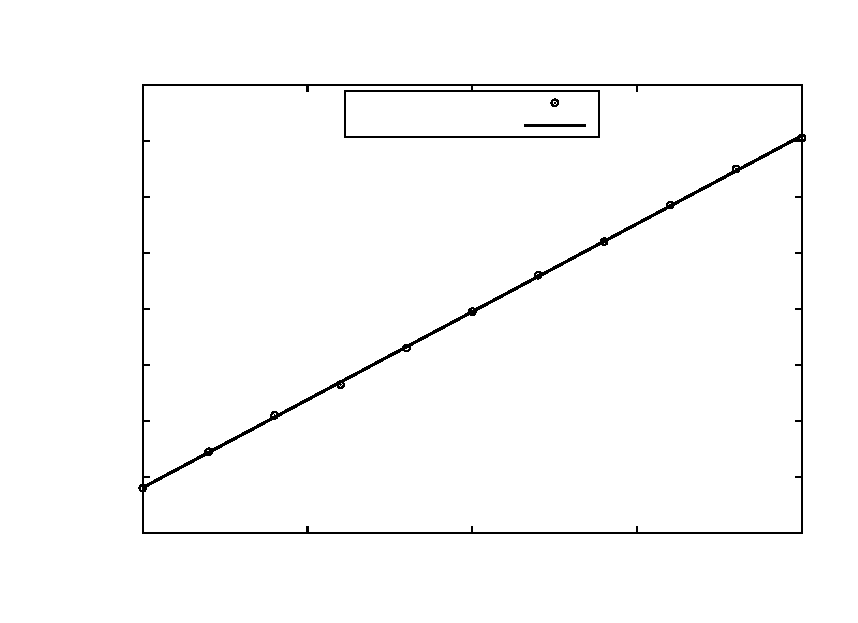
\includegraphics{graph-1}}%
    \gplfronttext
  \end{picture}%
\endgroup

        \caption{Dados do procedimento 1}
        \label{graph-1}  
    \end{subfigure}

    \begin{subfigure}[!htp]{0.3\textwidth}
        % GNUPLOT: LaTeX picture with Postscript
\begingroup
  \makeatletter
  \providecommand\color[2][]{%
    \GenericError{(gnuplot) \space\space\space\@spaces}{%
      Package color not loaded in conjunction with
      terminal option `colourtext'%
    }{See the gnuplot documentation for explanation.%
    }{Either use 'blacktext' in gnuplot or load the package
      color.sty in LaTeX.}%
    \renewcommand\color[2][]{}%
  }%
  \providecommand\includegraphics[2][]{%
    \GenericError{(gnuplot) \space\space\space\@spaces}{%
      Package graphicx or graphics not loaded%
    }{See the gnuplot documentation for explanation.%
    }{The gnuplot epslatex terminal needs graphicx.sty or graphics.sty.}%
    \renewcommand\includegraphics[2][]{}%
  }%
  \providecommand\rotatebox[2]{#2}%
  \@ifundefined{ifGPcolor}{%
    \newif\ifGPcolor
    \GPcolorfalse
  }{}%
  \@ifundefined{ifGPblacktext}{%
    \newif\ifGPblacktext
    \GPblacktexttrue
  }{}%
  % define a \g@addto@macro without @ in the name:
  \let\gplgaddtomacro\g@addto@macro
  % define empty templates for all commands taking text:
  \gdef\gplbacktext{}%
  \gdef\gplfronttext{}%
  \makeatother
  \ifGPblacktext
    % no textcolor at all
    \def\colorrgb#1{}%
    \def\colorgray#1{}%
  \else
    % gray or color?
    \ifGPcolor
      \def\colorrgb#1{\color[rgb]{#1}}%
      \def\colorgray#1{\color[gray]{#1}}%
      \expandafter\def\csname LTw\endcsname{\color{white}}%
      \expandafter\def\csname LTb\endcsname{\color{black}}%
      \expandafter\def\csname LTa\endcsname{\color{black}}%
      \expandafter\def\csname LT0\endcsname{\color[rgb]{1,0,0}}%
      \expandafter\def\csname LT1\endcsname{\color[rgb]{0,1,0}}%
      \expandafter\def\csname LT2\endcsname{\color[rgb]{0,0,1}}%
      \expandafter\def\csname LT3\endcsname{\color[rgb]{1,0,1}}%
      \expandafter\def\csname LT4\endcsname{\color[rgb]{0,1,1}}%
      \expandafter\def\csname LT5\endcsname{\color[rgb]{1,1,0}}%
      \expandafter\def\csname LT6\endcsname{\color[rgb]{0,0,0}}%
      \expandafter\def\csname LT7\endcsname{\color[rgb]{1,0.3,0}}%
      \expandafter\def\csname LT8\endcsname{\color[rgb]{0.5,0.5,0.5}}%
    \else
      % gray
      \def\colorrgb#1{\color{black}}%
      \def\colorgray#1{\color[gray]{#1}}%
      \expandafter\def\csname LTw\endcsname{\color{white}}%
      \expandafter\def\csname LTb\endcsname{\color{black}}%
      \expandafter\def\csname LTa\endcsname{\color{black}}%
      \expandafter\def\csname LT0\endcsname{\color{black}}%
      \expandafter\def\csname LT1\endcsname{\color{black}}%
      \expandafter\def\csname LT2\endcsname{\color{black}}%
      \expandafter\def\csname LT3\endcsname{\color{black}}%
      \expandafter\def\csname LT4\endcsname{\color{black}}%
      \expandafter\def\csname LT5\endcsname{\color{black}}%
      \expandafter\def\csname LT6\endcsname{\color{black}}%
      \expandafter\def\csname LT7\endcsname{\color{black}}%
      \expandafter\def\csname LT8\endcsname{\color{black}}%
    \fi
  \fi
  \setlength{\unitlength}{0.0500bp}%
  \begin{picture}(7936.00,5668.00)%
    \gplgaddtomacro\gplbacktext{%
      \csname LTb\endcsname%
      \put(682,704){\makebox(0,0)[r]{\strut{} 0}}%
      \put(682,1242){\makebox(0,0)[r]{\strut{} 1}}%
      \put(682,1780){\makebox(0,0)[r]{\strut{} 2}}%
      \put(682,2318){\makebox(0,0)[r]{\strut{} 3}}%
      \put(682,2856){\makebox(0,0)[r]{\strut{} 4}}%
      \put(682,3393){\makebox(0,0)[r]{\strut{} 5}}%
      \put(682,3931){\makebox(0,0)[r]{\strut{} 6}}%
      \put(682,4469){\makebox(0,0)[r]{\strut{} 7}}%
      \put(682,5007){\makebox(0,0)[r]{\strut{} 8}}%
      \put(1262,484){\makebox(0,0){\strut{}-800}}%
      \put(2159,484){\makebox(0,0){\strut{}-700}}%
      \put(3056,484){\makebox(0,0){\strut{}-600}}%
      \put(3952,484){\makebox(0,0){\strut{}-500}}%
      \put(4849,484){\makebox(0,0){\strut{}-400}}%
      \put(5746,484){\makebox(0,0){\strut{}-300}}%
      \put(6642,484){\makebox(0,0){\strut{}-200}}%
      \put(7539,484){\makebox(0,0){\strut{}-100}}%
      \put(176,2855){\makebox(0,0){\strut{}N}}%
      \put(4176,154){\makebox(0,0){\strut{}Pressão (mBar)}}%
      \put(4176,5337){\makebox(0,0){\strut{}Procedimento 2 - determinando $\frac{\triangle N}{\triangle p}$}}%
    }%
    \gplgaddtomacro\gplfronttext{%
      \csname LTb\endcsname%
      \put(4541,4834){\makebox(0,0)[r]{\strut{}dados}}%
      \csname LTb\endcsname%
      \put(4541,4614){\makebox(0,0)[r]{\strut{}fitting n(p)}}%
    }%
    \gplbacktext
    \put(0,0){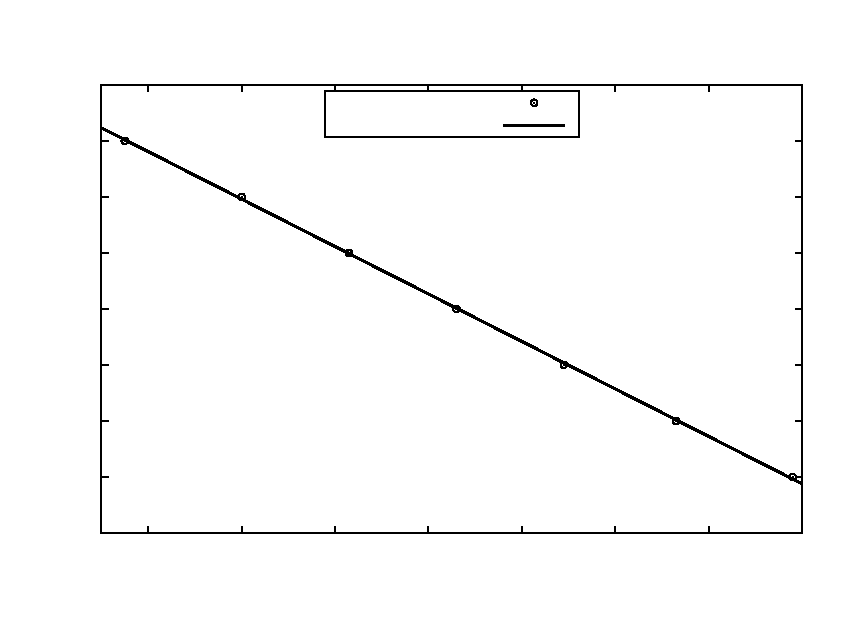
\includegraphics{graph-2}}%
    \gplfronttext
  \end{picture}%
\endgroup

        \caption{DADOSs do procedimento 1}
        \label{graph-2}  
    \end{subfigure}
    
    \caption{Gráficos}
    
\end{figure}


\FloatBarrier


%@@@@@@@@@@@@@@@@@@@@@@@@@@@@@@@@@@@@@@@@@@@@@@@@@@@@@@@@@@@
%@@@@@@@@@@@@@@       CONCLUSAO       @@@@@@@@@@@@@@@@@@@@@@
%@@@@@@@@@@@@@@@@@@@@@@@@@@@@@@@@@@@@@@@@@@@@@@@@@@@@@@@@@@@
\section{Conclusão}
\paragraph{} O experimento permitiu utilizar o interferômetro de Michelson para medir algumas constantes com grande precisão. Mediu-se o comprimento de onda do laser em estudo $\lambda = (628 \pm 2) \mbox{nm}$ e o índice de refração da luz a pressão ambiente $n = 1.000237 \pm 0.000002$. O valor obtido para $\lambda$ não bate com o valor nominal de 632nm e o erro esperado para n na ordem de $10^{-5}$. As medidas obtidas foram bastante precisas mas não acuradas. No cálculo do erro não foi considerado o erro aleatório, o que poderia aumentar a margem de erro e a acurácia das medidas. Por último, e quem sabe mais importante, a observação do efeito de interferência demonstra o caráter ondulatório da luz.
%@@@@@@@@@@@@@@@@@@@@@@@@@@@@@@@@@@@@@@@@@@@@@@@@@@@@@@@@@@@
%@@@@@@@@@@@@@@       REFERÊNCIAS     @@@@@@@@@@@@@@@@@@@@@@
%@@@@@@@@@@@@@@@@@@@@@@@@@@@@@@@@@@@@@@@@@@@@@@@@@@@@@@@@@@@
\begin{thebibliography}{9}    
	 \bibitem{fis4-serway}
  		JEWETT, J.W.; SERWAY, R.A.
  		\emph{Física para cientistas e engenheiros} volume 4 : Luz, Óptica e Física Moderna.
 		 8ª ed.
 		 São Paulo : Cengage Learning, 2012.
\end{thebibliography}
\end{document}
